\subsection{Error Evaluation}
To improve length estimation accuracy, we expanded Eq. (\ref{eq:model}) by adding the terms $p^2$ and $d^2$ and increasing the parameters as follows:
\begin{equation}
\label{eq:model_2d(1)}
F = (b_5p^2 + b_4pd + b_3d^2 + b_2p+b_1d+b_0)d
\end{equation}
As a result, with respect to the measurements by the linear encoder,the dynamic length estimation was achieved with the maximum errors of $1.12\%$ for PAM-A, $0.773\%$ for PAM-B, $1.01\%$ for PAM-B, and $0.755\%$ for PAM-D respectively, and with the root mean squared errors of $0.633\%$ for PAM-A, $0.353\%$ for PAM-B, $0.548\%$ for PAM-C, and $0.435\%$ for PAM-D respectively. The errors were reduced as expected for all PAMs. 
% As a result, the dynamic length estimation was achieved with maximum errors within $1.12\%$ and mean squared error rates within $0.633\%$, and the errors were reduced as expected for all PAMs. 

% As a result, as shown in the third and fourth columns of Table \ref{tab:error}, the errors were reduced as expected for all PAMs. 

We also tried another approach by introducing a cubic polynomial model and increasing the parameters as follows:
\begin{equation}
    \label{eq:model_3d}
    F = (c_4p^3+c_3p^2d+c_2pd^2+c_1d^2+c_0)d
\end{equation}
As predicted, the root mean squared errors decreased to $0.516\%$ for PAM-A, $0.484\%$ for PAM-B, $0.500\%$ for PAM-C, and $0.606\%$ for PAM-D respectively. 
However, even though the maximum errors decreased to $1.22\%$ for PAM-A and $0.951\%$ for PAM-C respectively, they actually increased to $1.41\%$ for PAM-B and $1.99\%$ for PAM-D respectively. This result suggests that, even if the coefficients of the model equation are determined experimentally, the degrees must be carefully determined based on previous studies so as to express intrinsic characteristics of the PAM. For example, the newly added term $p^3$ may have amplified the error of the pressure sensor. When applying our model to a reflex mechanism, it will also be necessary to carefully consider the contribution of each term to the accuracy of the length estimation based on the reliability of the force and pressure sensors used.

Wickramatunge et al. proposed separating the parameters $a_i$ into contraction ones $a^c_i$ and extension ones $a^e_i$ to reflect the hysteresis of the PAM\cite{spring}. They also suggested using different parameters for low-pressure and high-pressure ranges to further improve the accuracy. However, our model ignores these suggestions and simplifies the length estimation method by using the same parameters across the entire pressure range, regardless of contraction or expansion. This is because our model is supposed to be applied to the reflex 

% \begin{figure}[H]
%     \hfill
%     \begin{minipage}{\columnwidth}
%         \centering
%         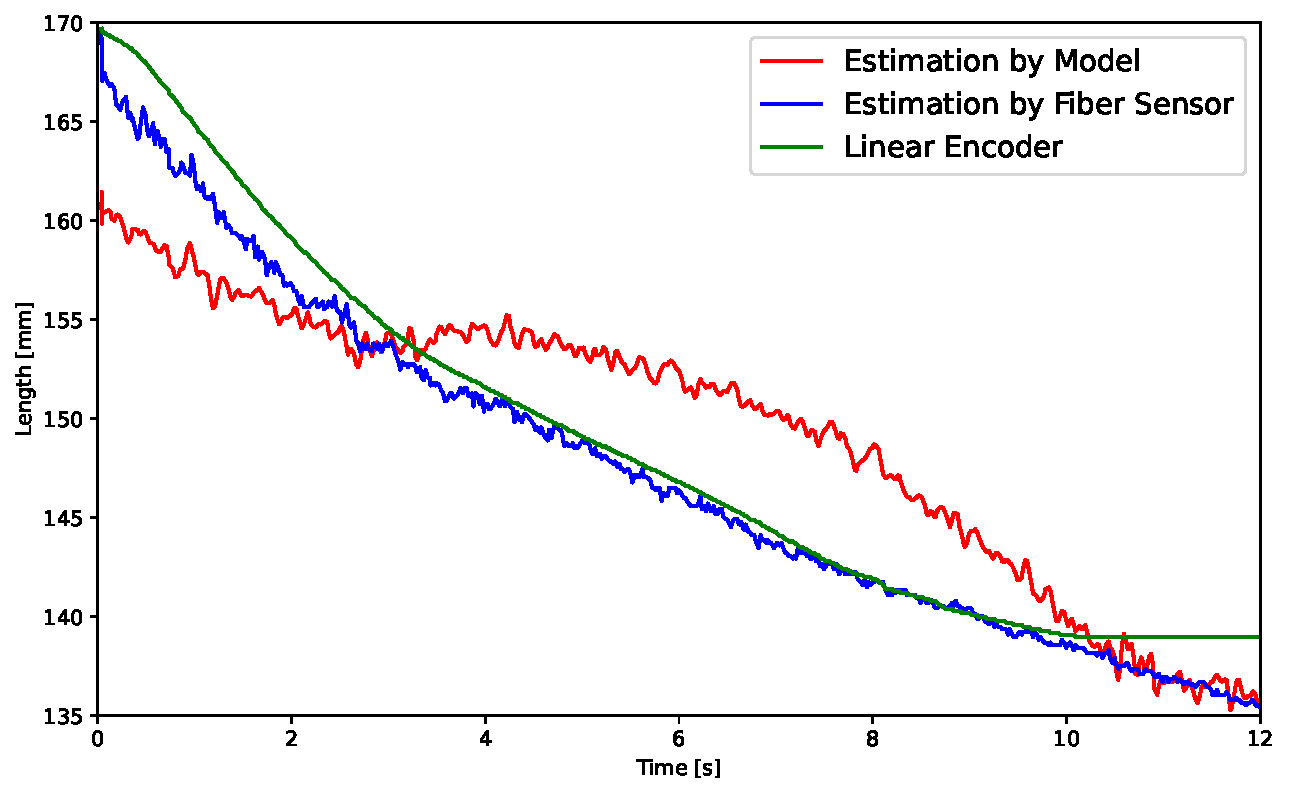
\includegraphics[width=\columnwidth]{fig/reaching_error.pdf} 
%         \caption{Relationship between Pressure and Natural Length}
%         \label{fig:length_pressure}
%         \vspace{1em} 
%         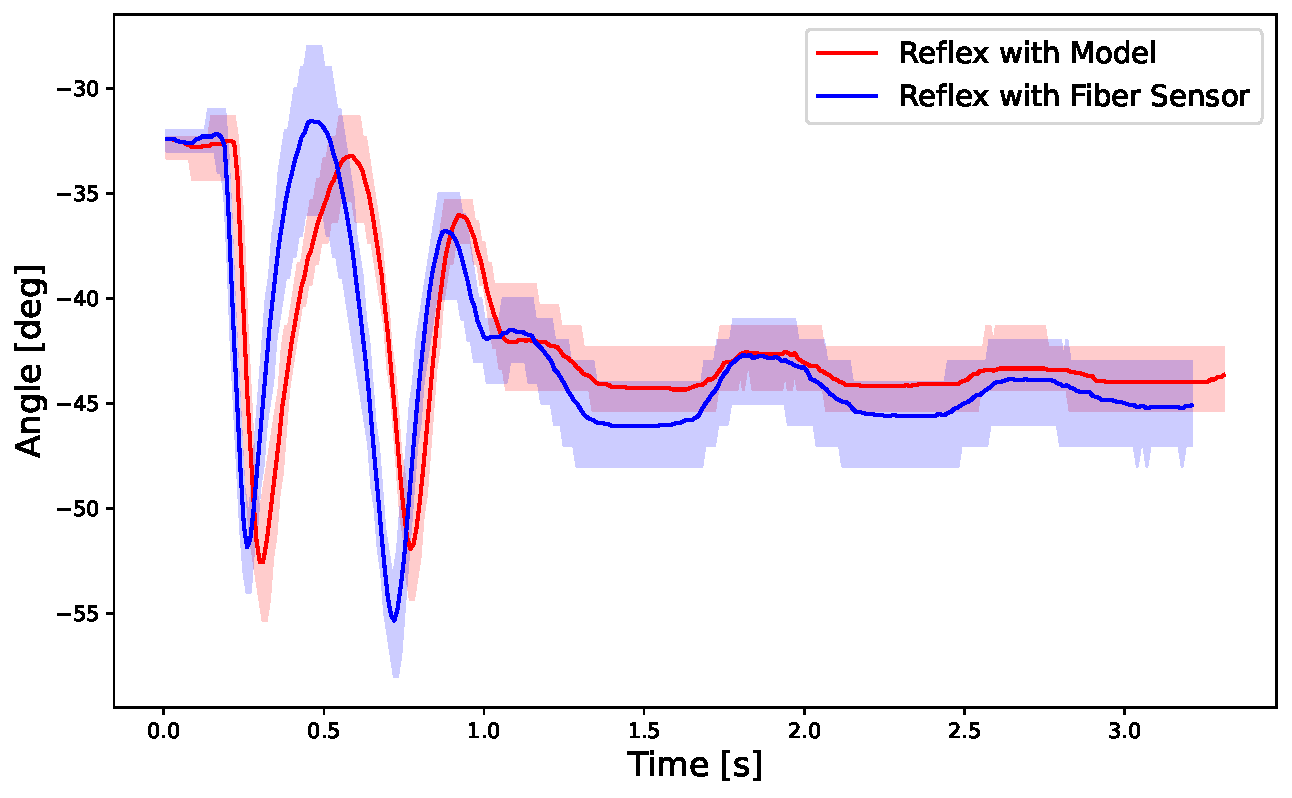
\includegraphics[width=\columnwidth]{fig/time_vs_angle_model_sensor.pdf}
%         \caption{Relationship between Force and Deformation at Each Pressure (PAM-B)}
%         \label{fig:pam_b_static1}
%     \end{minipage}
%     \hspace{0.05\textwidth} 
% \end{figure}

\begin{figure*}[t]
    \centering
    \begin{minipage}[H]{\textwidth} % 全幅を使用
        \begin{minipage}[H]{0.48\textwidth} % 左側の半分
            \centering
            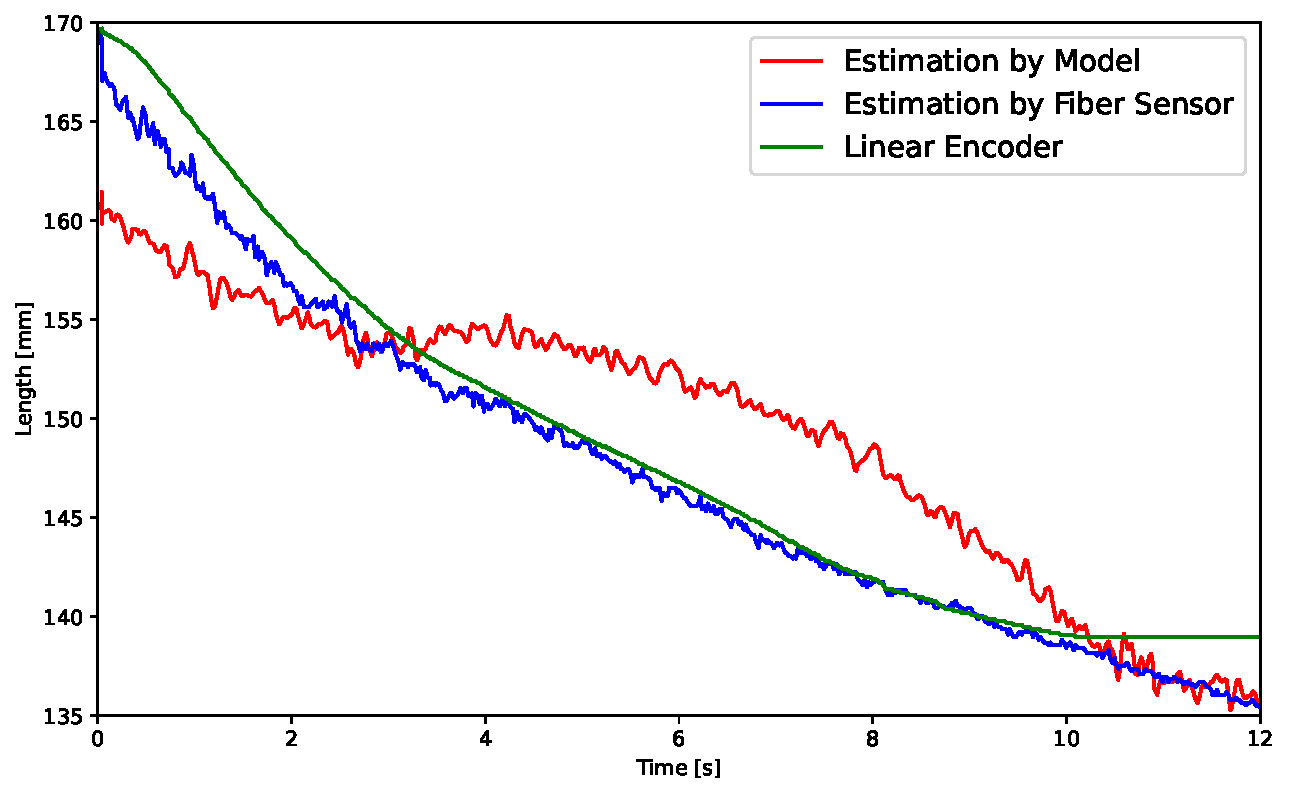
\includegraphics[width=\columnwidth]{fig/reaching_error.pdf}
            \caption{Length Estimation Error in Reaching Task}
            \label{fig:reaching_error}
            \vspace{1em}
            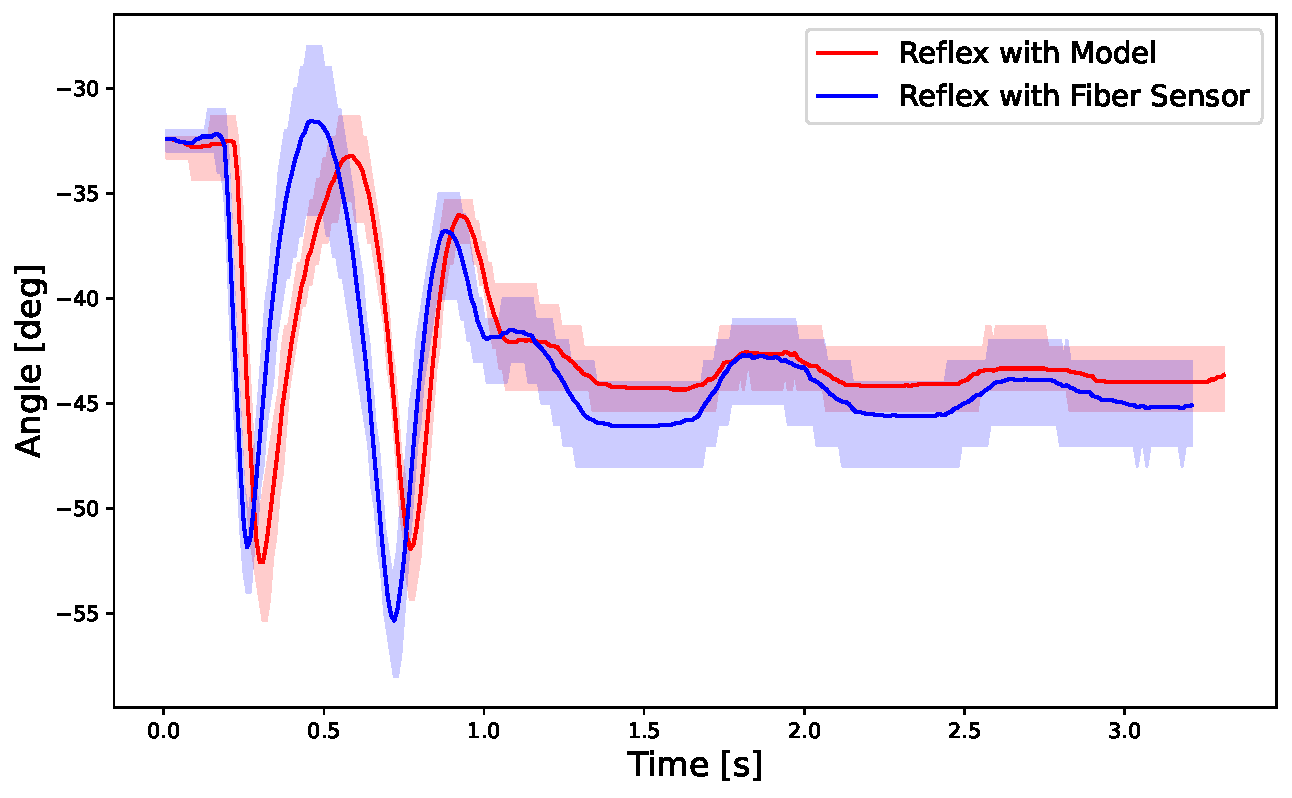
\includegraphics[width=\columnwidth]{fig/time_vs_angle_model_sensor.pdf}
            \caption{Comparison of Reflex Angles between Model and Fiber Sensor }
            \label{fig:reflex_angle}
        \end{minipage}
        \hfill
        \begin{minipage}[H]{0.48\textwidth} % 右側の半分
            \centering
            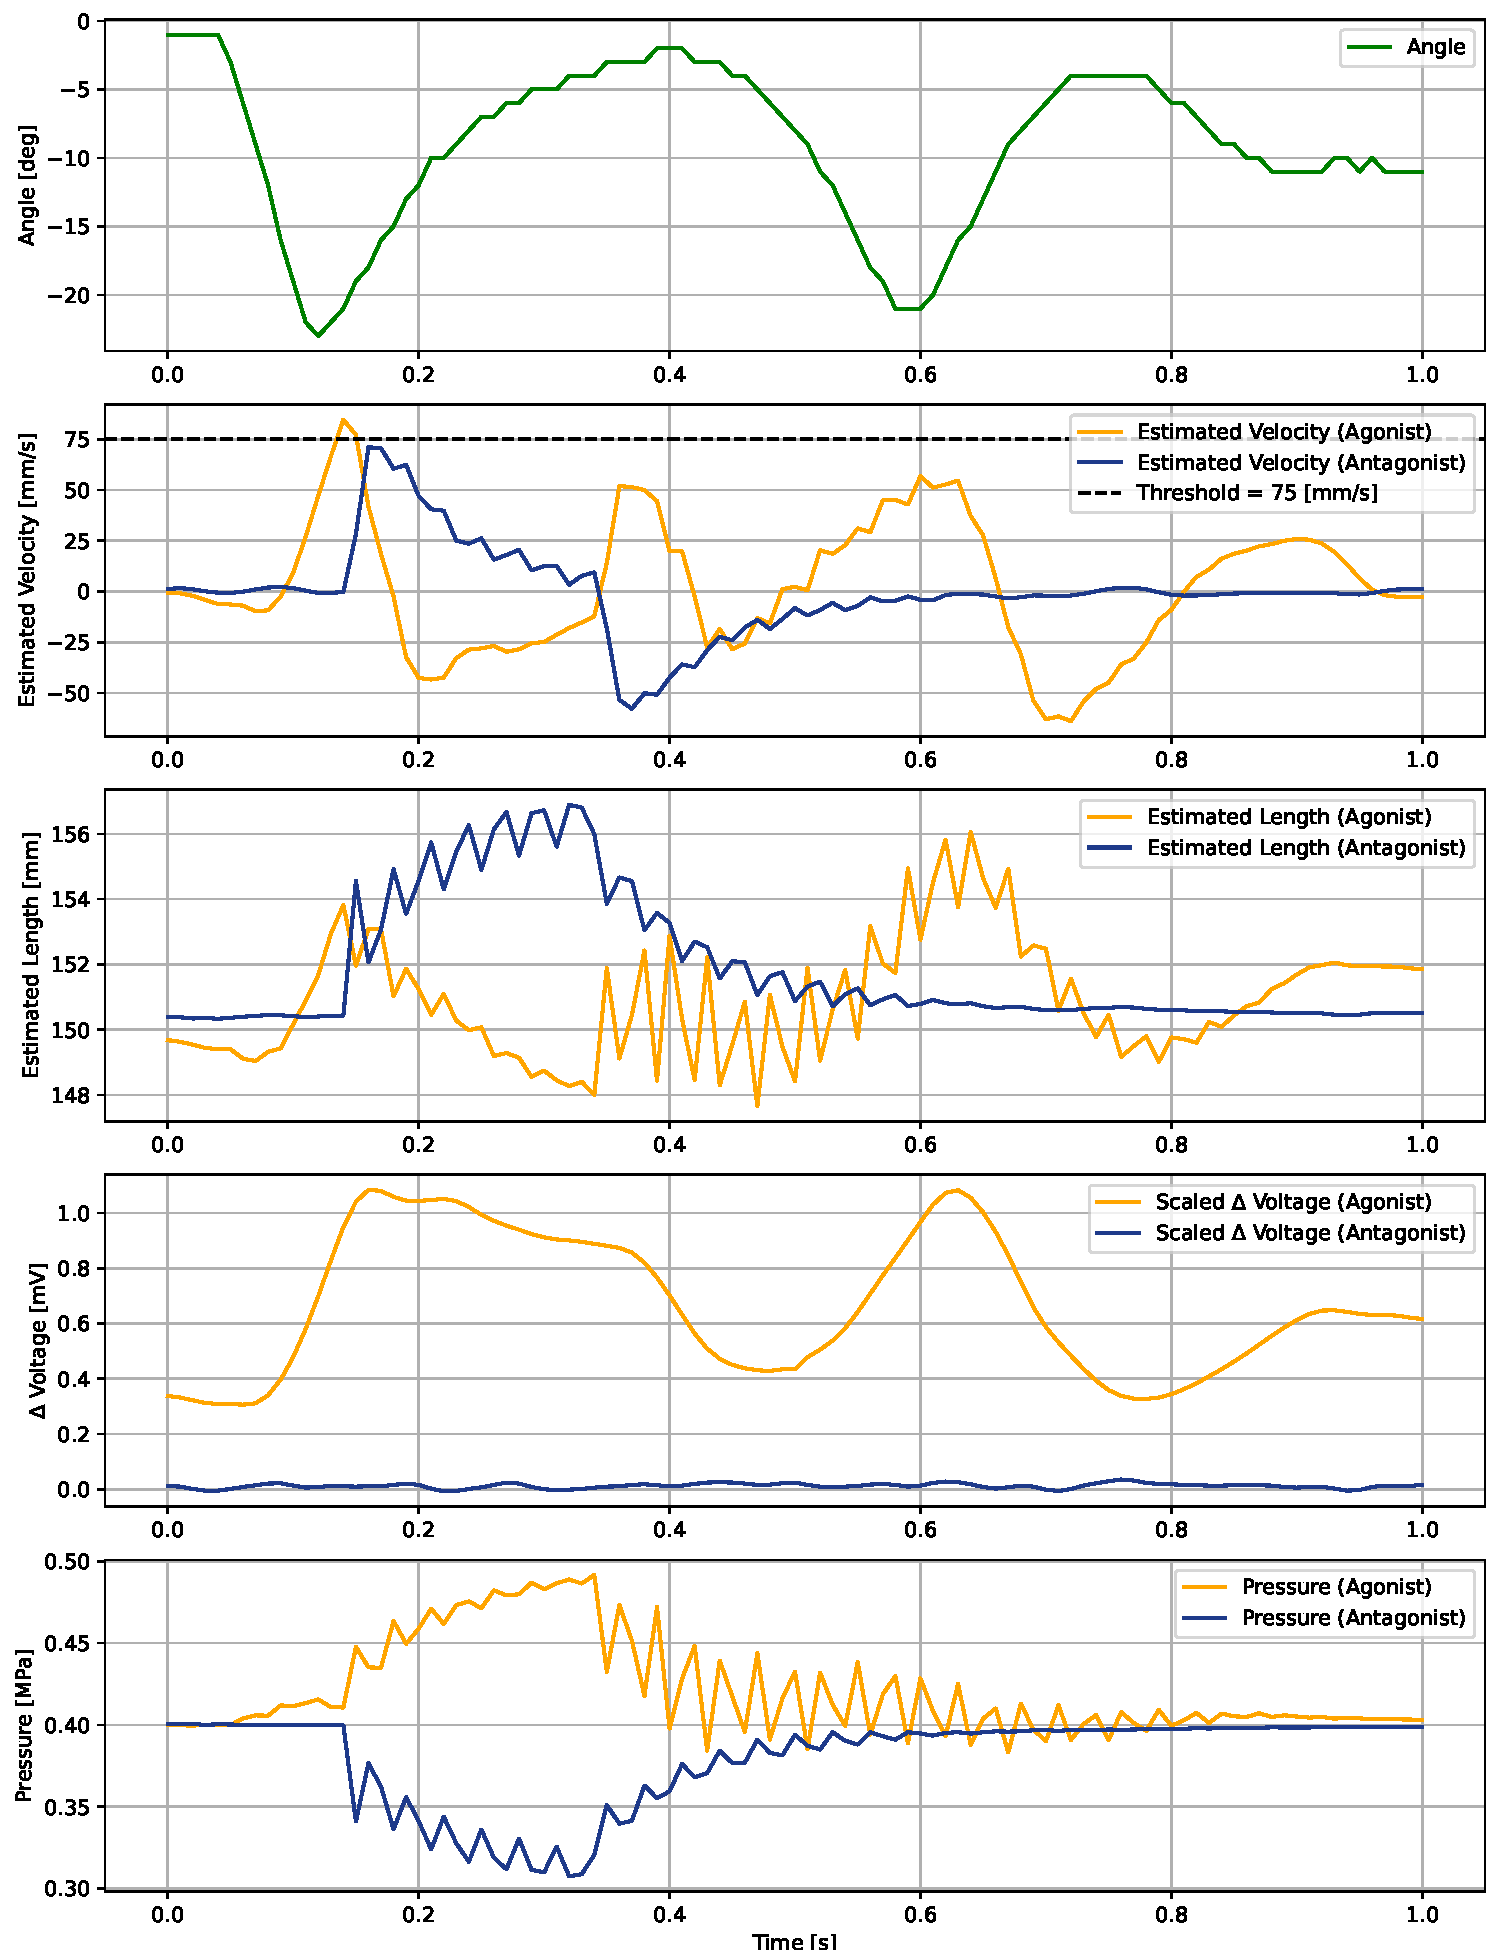
\includegraphics[width=\columnwidth]{fig/20240819_r20_reflex_all_plt.pdf}
            \caption{Dynamic Reflex Behavior of Agonist and Antagonist Muscles}
            \label{fig:reflex_all}
        \end{minipage}
    \end{minipage}
\end{figure*}

\noindent mechanism. If the parameters have to be switched depending on the situation, it would be difficult for the reflex mechanism to respond quickly to disturbances.
% Additionally, since the reflex mechanism is only required to detect sudden extension or contraction of the PAM, a minor decrease in precision is acceptable. 
% The reflex mechanism aims to reduce the computational load on the central control system, so the computational load ot the reflex mechanism itself must not be high. 
Musculoskeletal robots often carry microcomputers on their structures, so the employed length estimation method is desired to be simple for efficient operation given the limited computational resources.



% \begin{figure}[h]
%     \centering
%     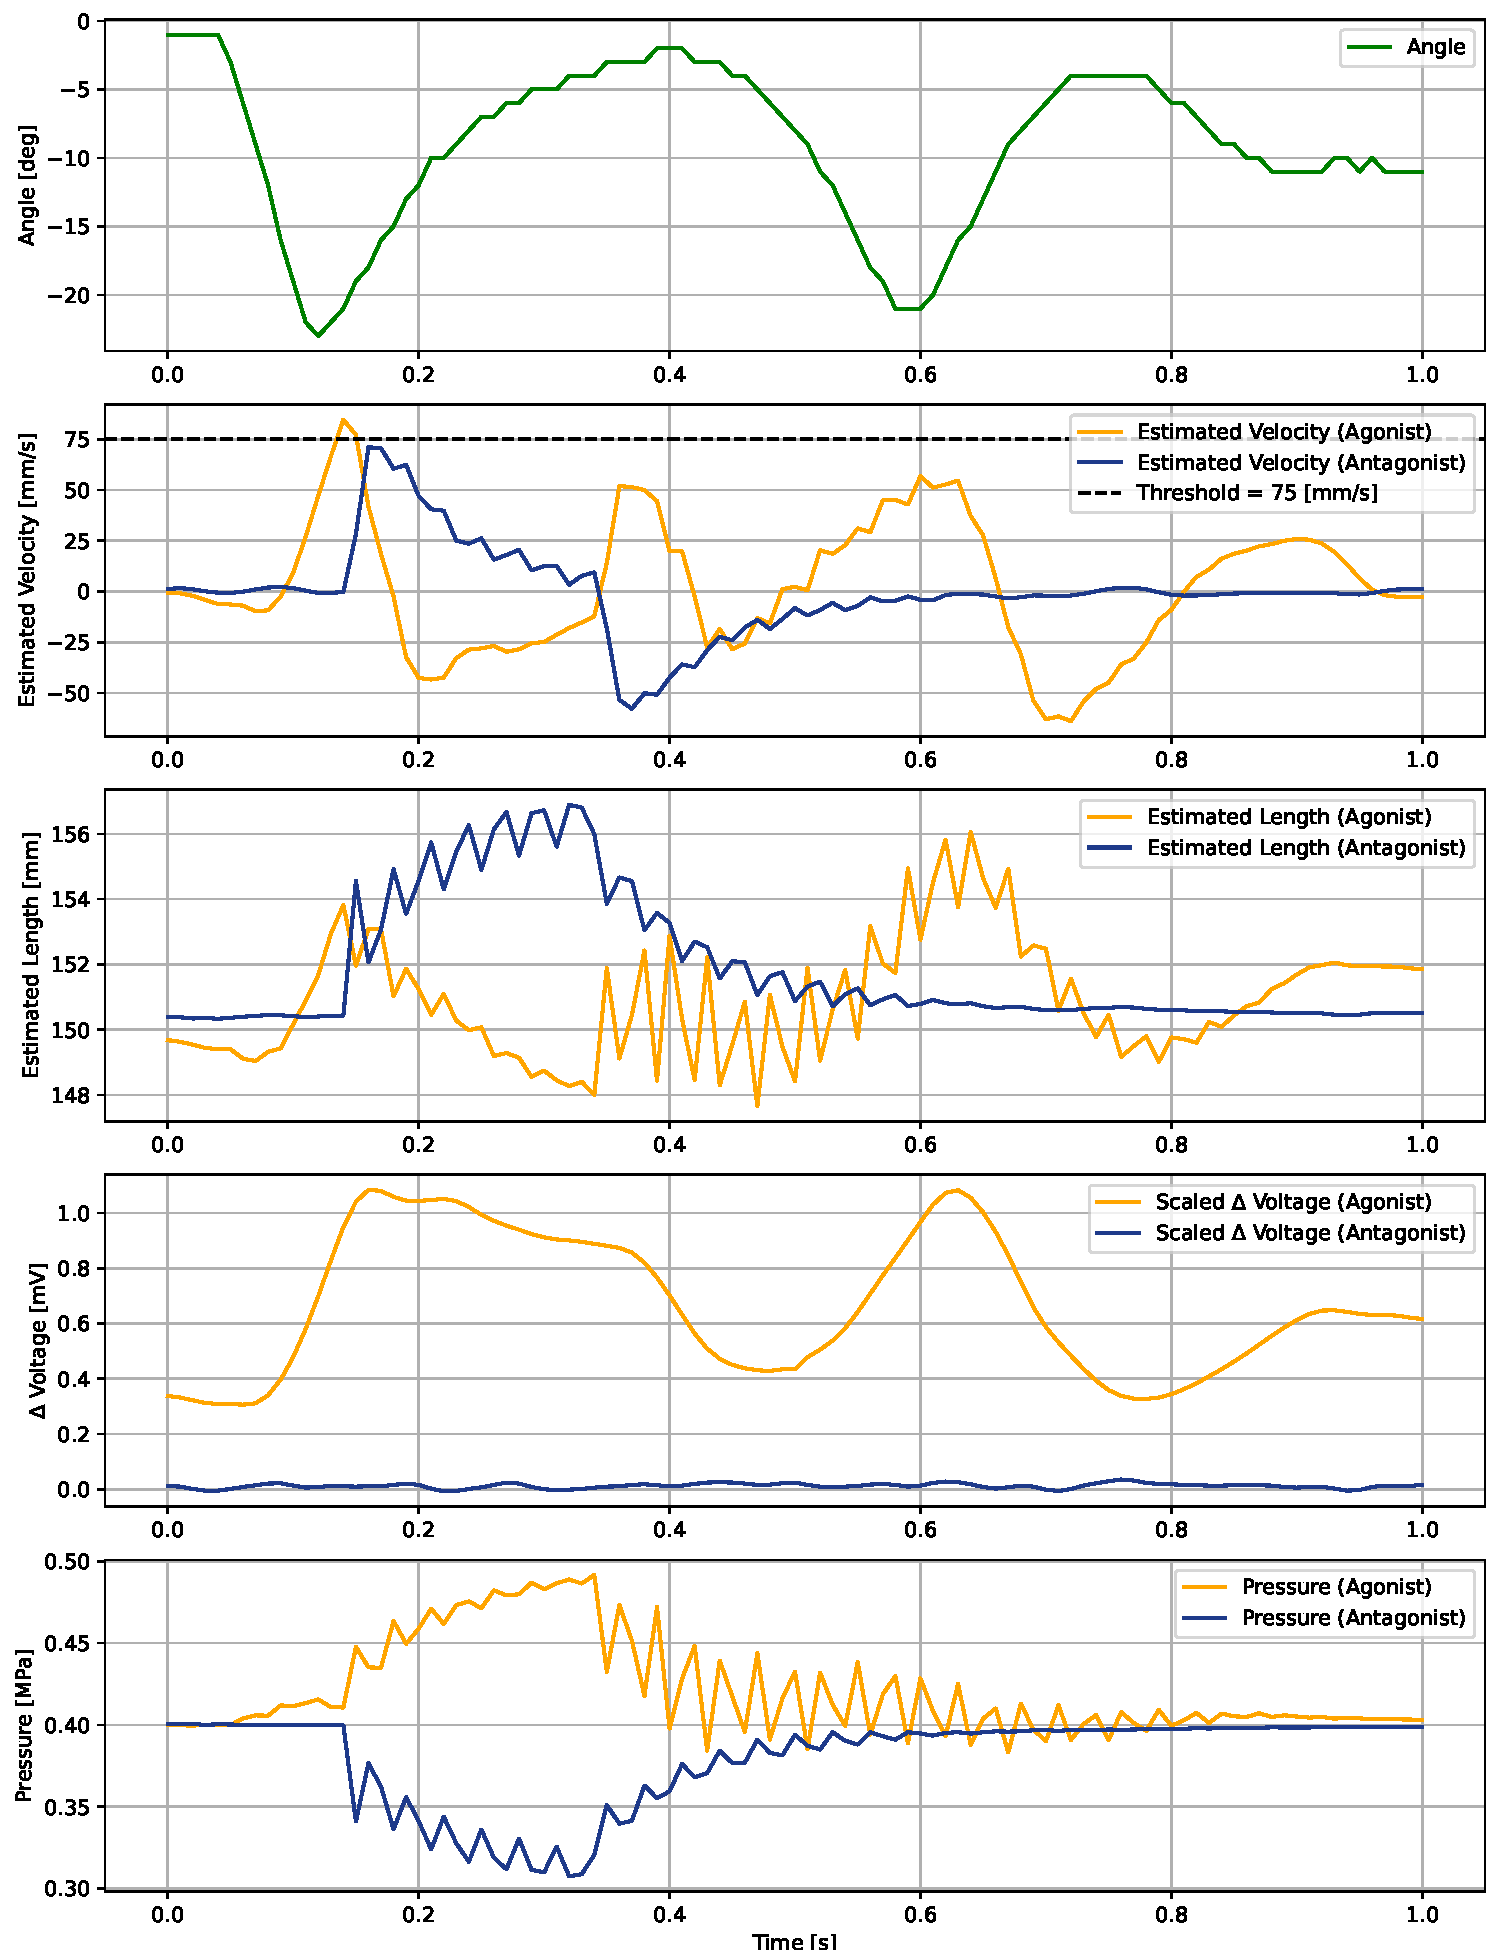
\includegraphics[width=\columnwidth]{fig/20240819_r20_reflex_all_plt.pdf}
%     \caption{Outline Diagram of Static Loading Experiment}
%     \label{fig:static_equipment}
%  \end{figure}

% \begin{figure*}[t] % figure* は twocolumn の場合、2カラム全体を使う
%     \centering
%     \begin{minipage}[t]{\columnwidth}
%         \centering
%         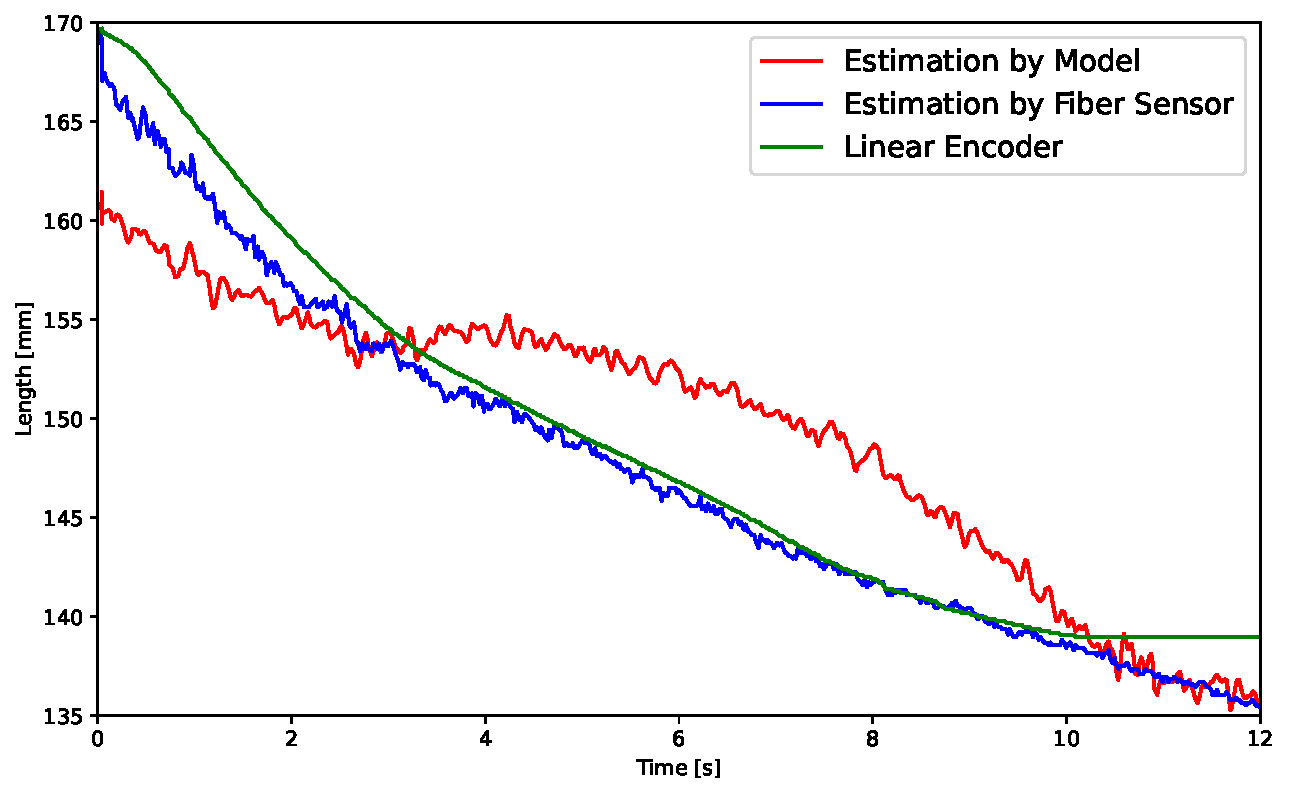
\includegraphics[width=\columnwidth]{fig/reaching_error.pdf}
%         \vspace{0.3cm}
%         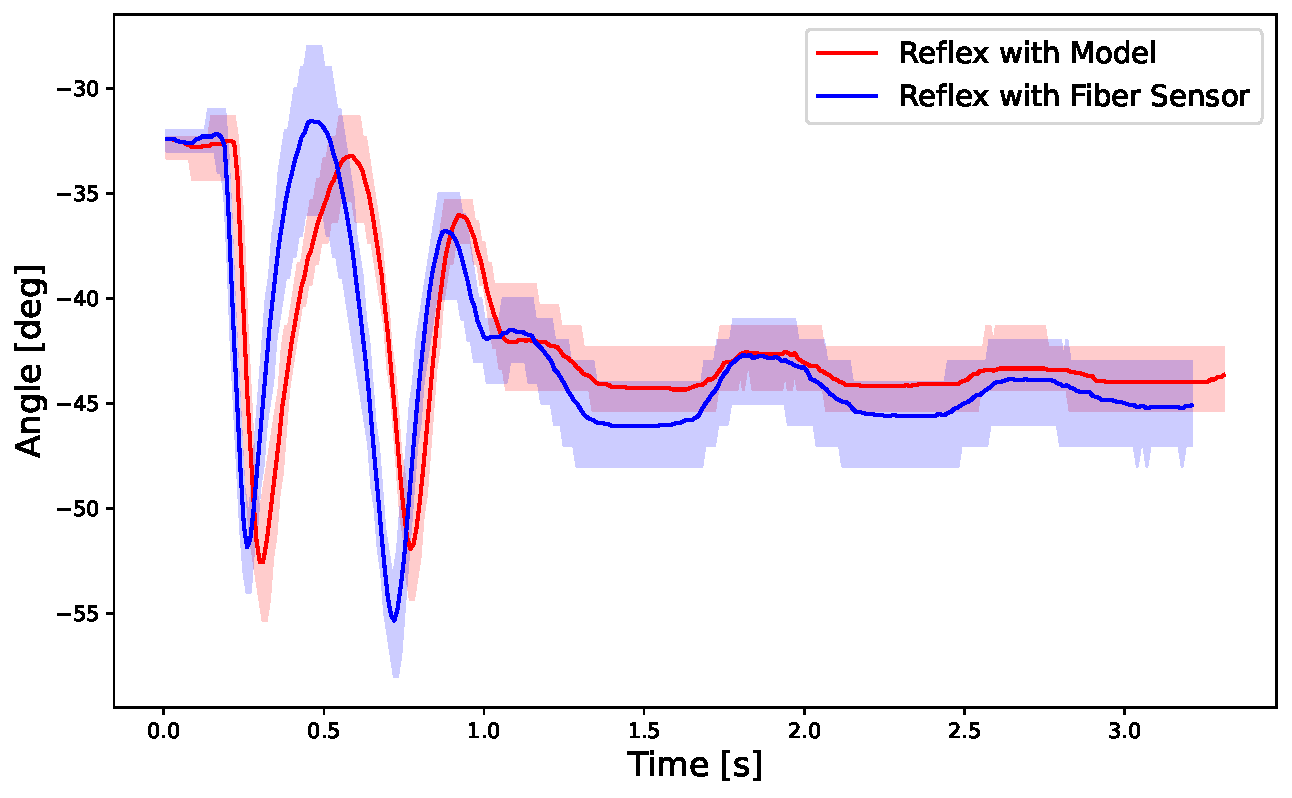
\includegraphics[width=\columnwidth]{fig/time_vs_angle_model_sensor.pdf}
%     \end{minipage}
%     \hfill
%     \begin{minipage}[t]{\columnwidth}
%         \centering
%         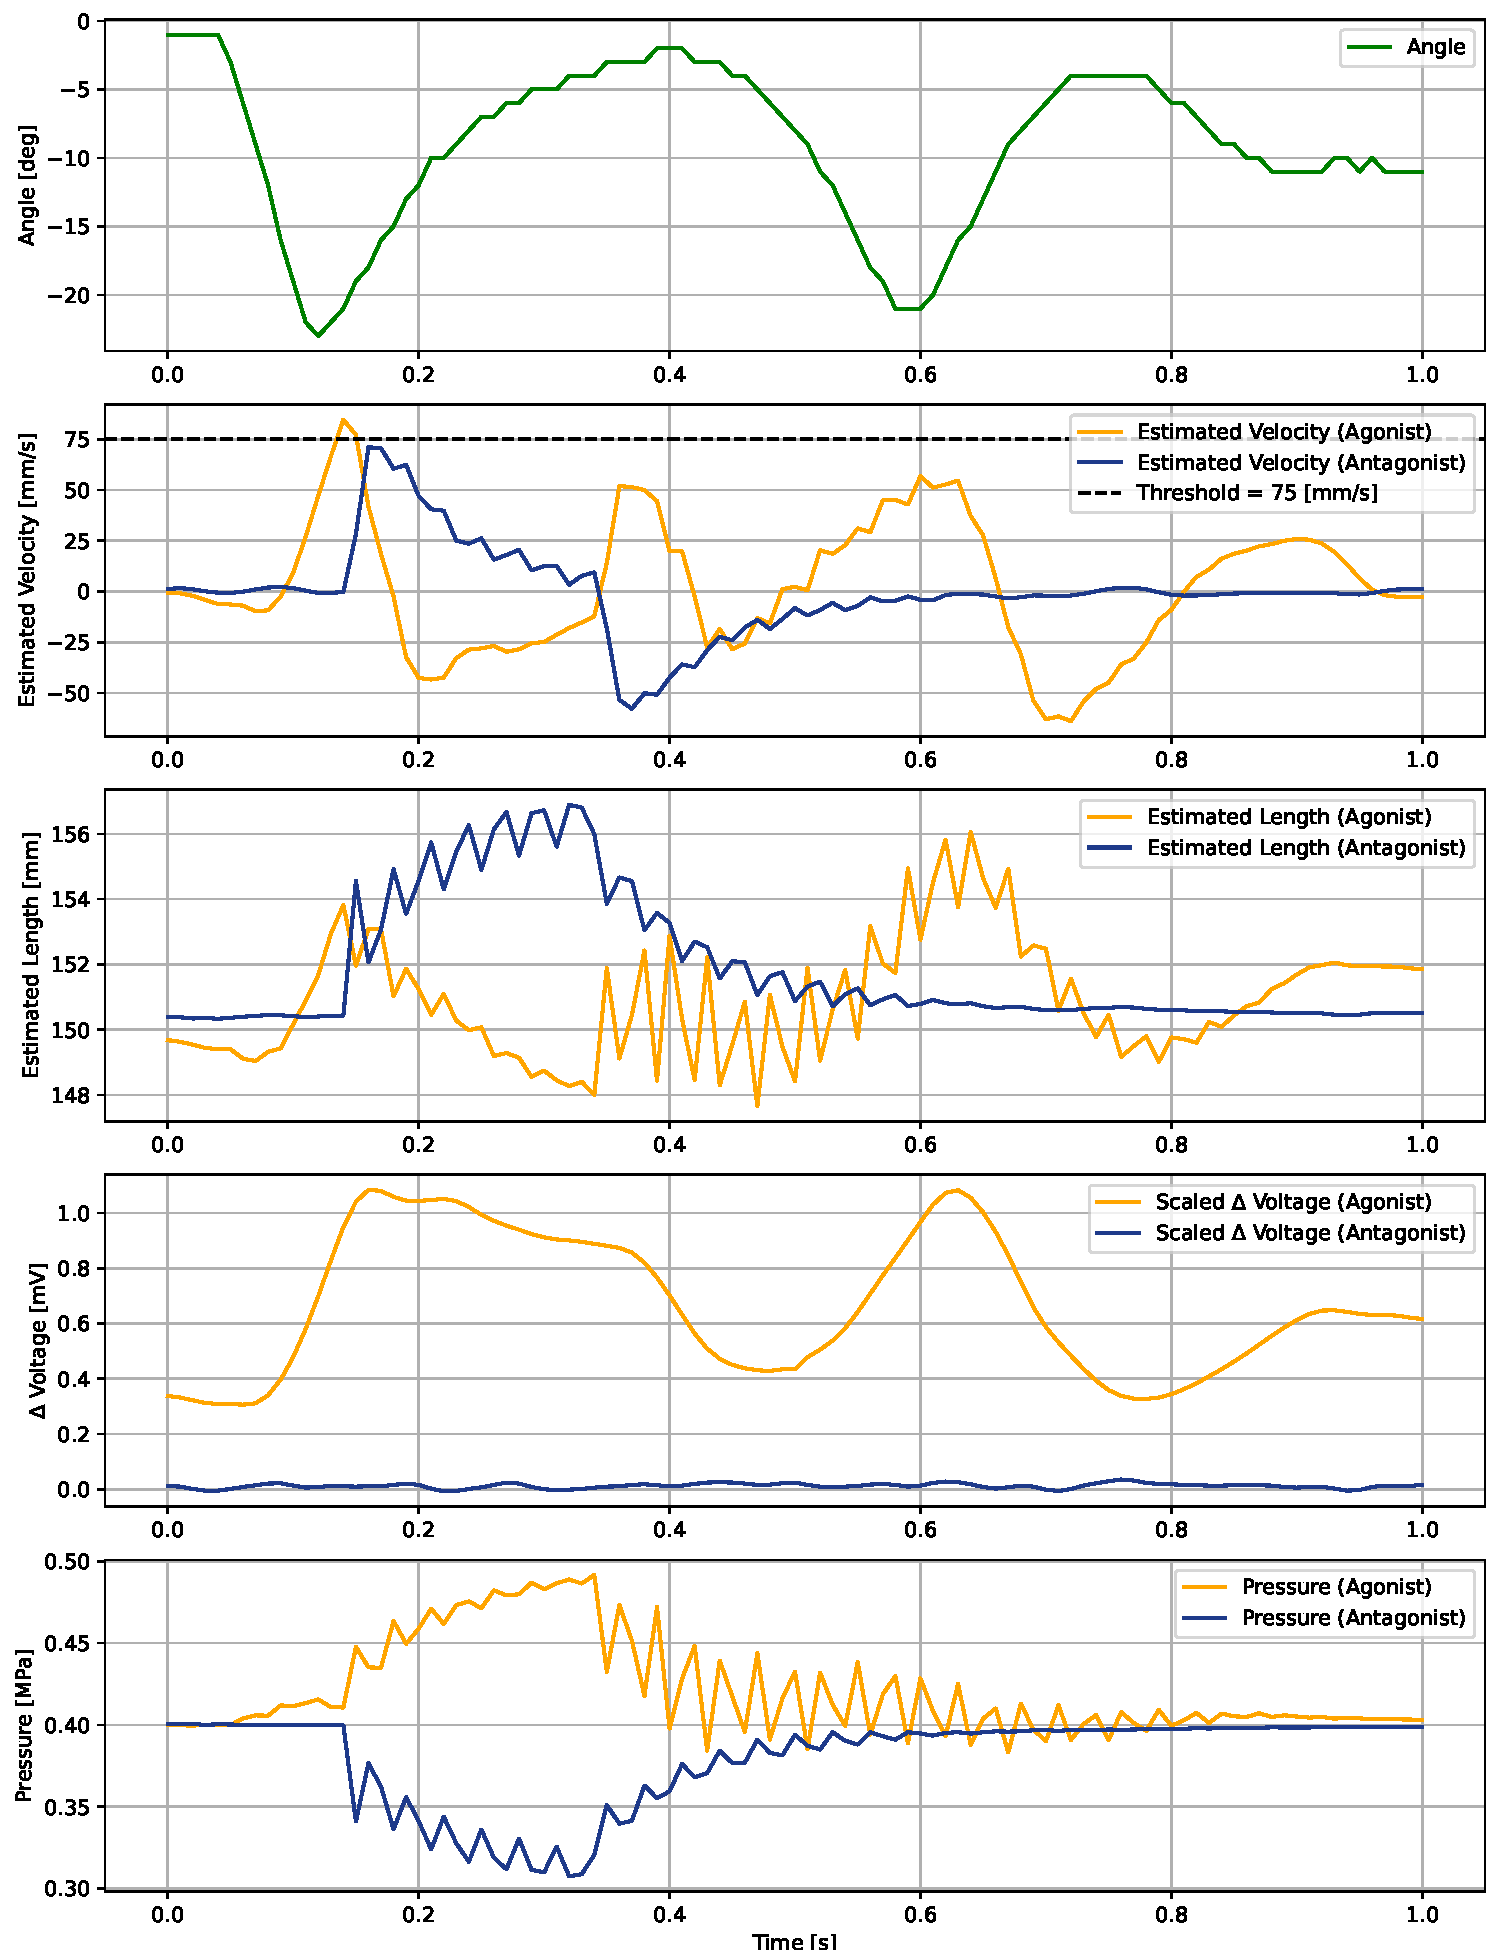
\includegraphics[width=\columnwidth]{fig/20240819_r20_reflex_all_plt.pdf}
%     \end{minipage}
%     \caption{a}
%     \label{fig:plots}
% \end{figure*}



\subsection{Reaching task}
\subsection{Stretch Reflex}

\newpage


% なお,WickramatungeらはPAMのヒステシスをモデルに反映させるために,推定パラメータ$a_i$を収縮時のパラメータ$a^c_i$と膨張時のパラメータ$a^e_i$に分けることを提案している.また,更に精度を向上させるために,低圧帯と高圧帯でもパラメータを使い分けることを提案している.本論文では,これらの提案を無視し,収縮・膨張を問わず全圧力範囲で同一のパラメータを用いることで,長さ推定の手法を単純化している.これは,本モデルによるPAMの長さ推定を反射機構に適用することを想定しているからである.推定パラメータを状況により切り替える必要があると,反射機構が外乱に迅速に反応することが困難になる.また,反射機構にはPAMの突然の伸長もしくは収縮を検知することだけが求められているので,PAMの精密な制御に求められるような高精度さは必要ないと考える.反射機構は中央制御系の計算負荷を軽減することを目的とするため,反射機構の計算負荷自体が高くてはならない.特に,筋骨格ロボットにはマイクロコンピュータを搭載することも多いため,計算資源の限られた環境での実行を考慮して,モデルを単純化している.
 


% To reduce the error in the length estimation, we expanded the spring constant in Equation (\ref{eq:model}) to a cubic polynomial of pressure $P$ and deformation $L_d$ and increased the number of the parameters as follows:

% \begin{equation}
% \label{eq:model_2d(1)}
% F = (b_5P^2 + b_4PL_d + b_3L^2_d + b_2P+b_1L_d+b_0)L_d
% \end{equation}

% Consequently, in some cases, the errors were actually increased as indicated in the third and fourth columns of Table \ref{tab:error}. This may be due to overfitting caused by an excessive increase in the parameters.
% In order to improve the accuracy of length estimation while avoiding overfitting to errors, it is necessary to investigate the contribution of each term of the spring constants in equations (\ref{eq:model}) and (\ref{eq:model_3d}) to fitting and to verify whether each term should be removed or added. The effect of each term during length estimation also depends on the reliability of a pressure sensor and a force sensor. For example, if the error of a pressure sensor is very small, adding the term $a_4P^3$ to the spring constants in equation (\ref{eq:model}) may reduce the error.

% \begin{equation}
%     \label{eq:model_3d}
%     F = (c_4P^3+c_3P^2L_d+c_2PL^2_d+c_1L^2_d+c_0)L_d
% \end{equation}
    
% 提案モデルによる長さ推定の誤差を低減しようと,(\ref{eq:model})式のバネ定数を
% \begin{equation}
% \label{eq:model_3d}
% F = (a_4P^3 + a_3P^2L_d + a_2PL^2_s + a_1L_d^3 +a_0)L_d
% \end{equation}
% のように,圧力$P$と変形量$L_d$の三次式にし,推定パラメータの数を増やした.
% その結果,表\ref{tab:error}の第4列および第5列に示すように,かえって誤差を増大させる場合があった.
% この原因として,過剰に推定パラメータを増やしたことで,誤差に対してオーバーフィティングするようになったことが考えられる.
% 誤差に対するオーバーフィッティングを防ぎつつ,長さ推定の精度を上げるには,
% (\ref{eq:model})式および(\ref{eq:model_3d})式のバネ定数の各項のフィッティングへの寄与を一つづつ調査し,
% 各項を削除もしくは追加するかを検証する必要がある.
% 長さ推定時の各項の効果には,圧力センサや力センサの信頼性も影響する.
% 例えば,圧力センサの誤差が非常に小さい場合,(\ref{eq:model})式のバネ定数に$a_4P^3$の項のみ追加すれば,
% 長さ推定の誤差が低減される可能性がある.

% \begin{table}[h]
%     \centering
%     \caption{Maximum error and root mean squared \\percentage error of dynamic length estimation }
%     \resizebox{\columnwidth}{!}{
%         \begin{tabular}{c|ccccccc}
%             \hline
%             PAM & \begin{tabular}[c]{@{}c@{}}Maximum Error[$\%$]\\(Eq.(\ref{eq:model})) \end{tabular} & \begin{tabular}[c]{@{}c@{}}Root Mean\\Squared Error[$\%$]\\(Eq.(\ref{eq:model})) \end{tabular} & \begin{tabular}[c]{@{}c@{}}Maximum Error[$\%$]\\(Eq.(\ref{eq:model_2d(1)})) \end{tabular} & \begin{tabular}[c]{@{}c@{}}Root Mean\\Squared Error[$\%$]\\(Eq.(\ref{eq:model_2d(1)})) \end{tabular}&\begin{tabular}[c]{@{}c@{}}Maximum Error[$\%$]\\(Eq.(\ref{eq:model_3d})) \end{tabular}&\begin{tabular}[c]{@{}c@{}}Root Mean\\Squared Error[$\%$]\\(Eq.(\ref{eq:model_3d})) \end{tabular} \\
%             \hline \hline
%             A & 1.72&0.861&1.12&0.633&1.22&0.516&\\
%             B & 1.19&0.653 &0.773&0.353&1.41&0.484&\\
%             C & 1.18&0.683&1.01&0.548&0.951&0.500&\\
%             D & 1.65 & 0.846 &0.755& 0.435&1.99&0.606&\\
%             \hline
%         \end{tabular}
%     }
%     \label{tab:error}
% \end{table}
